\documentclass[UTF8]{ctexart}
\usepackage{graphicx}
\usepackage{float}
\usepackage{geometry}
\usepackage{fancyhdr}
\usepackage{lastpage}
\usepackage{amsmath}
\usepackage{mathrsfs}
\usepackage{amsthm}
\usepackage{multicol}
\usepackage{multirow}
\usepackage{subfigure}
\usepackage[colorlinks,linkcolor=black]{hyperref}
\geometry{left=2.54cm,right=2.54cm,top=3.18cm,bottom=3.18cm}%页边距
\pagestyle{fancy}
\lhead{
\includegraphics[scale=1]{sjtu-logo-red.pdf}}  
\rhead{CT成像的扫描与重建算法实现} 
\cfoot{第 \thepage\ 页\ 共 \pageref{LastPage} 页} 
\newtheorem{theorem}{定理}

\begin{document}

\begin{titlepage}
    \begin{center}
        
\includegraphics[width=0.8\textwidth]{sjtu-name-blue.pdf}\\[1cm]
        \textsc{\Huge \bfseries 课程报告}\\[1.5cm]
        
\includegraphics[width=0.3\textwidth]{sjtu-badge-blue.pdf}\\[0.5cm]    

        \Huge \bfseries{CT成像的扫描与重建算法实现}\\[1cm]
        \LARGE \bfseries{生物医学图像处理(2)课程作业}\\[1cm]
        \Large \bfseries{518021910971 裴奕博}
    \end{center}
\end{titlepage}
\tableofcontents
\newpage

%正文
\section{项目背景}

\subsection{CT重建算法}
自20世纪70年代被发明以来,X射线计算机断层成像(CT)在医学影像检查中扮演了越来越重要的地位。在CT成像的流程中,将图像进行数字化、投影和重建的算法非常重要。CT成像算法的好坏,会直接影响到CT的成像质量。

\subsection{数学基础}
中心切片定理和滤波反投影算法的提出,是CT成像和重建算法的数学基础。

中心切片定理可以表述如下:
\begin{theorem}[中心切片定理]
    $$P(\omega,\theta)=F(\omega\cos\theta,\omega\sin\theta)$$
    其中P是投影函数$p(l,\theta)$的傅里叶变换,$F(u,v)$是图像的
    二维傅里叶变换。
\end{theorem}
该定理说明,某断层在角度为$\theta$时得到的平行投影的一维傅里叶变换,等于图像二维傅里叶变换过原点的一个垂直切片,且切片的方向也为$\theta$角。

通过中心切片定理,我们可以得到原CT图像的投影图,再经过重建算法就可以得到CT重建图像。重建算法主要分为两大类:滤波反投影算法和反卷积反投影算法。本次的重建算法属于滤波反投影算法,可以用公式表示如下:

\begin{theorem}[滤波反投影算法]
    $$f(x,y)=\int_0^{\pi}|\omega|P(\omega,\theta)\exp(j2\pi\omega l)\lvert_{l=x\cos\theta+y\sin\theta}$$
\end{theorem}
其中$P(\omega,\theta)$是通过中心切片定理得到的投影图的傅里叶变换。

\section{项目实现}
\subsection{项目总体实现}
项目的整体流程比较简单,如下图:

\begin{figure}[H]
    \centering
    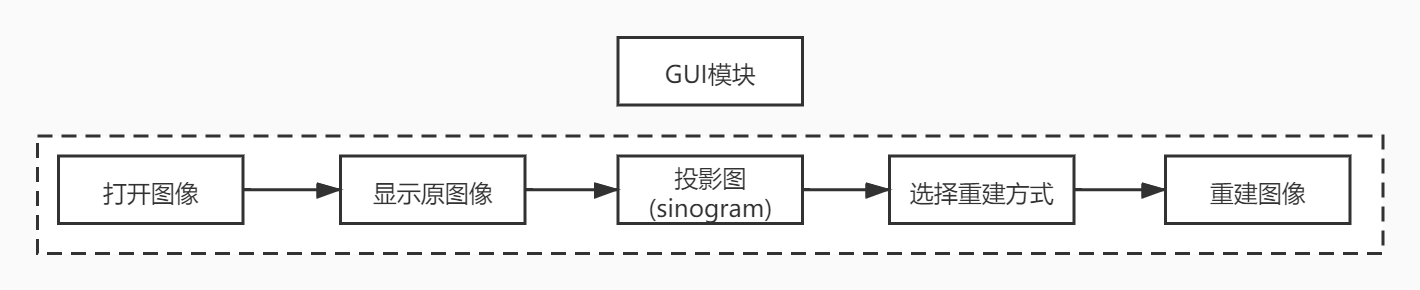
\includegraphics[width=\textwidth]{../image/workflow.jpg}
    \caption{项目流程图}
    \label{fig workflow}
\end{figure}
所有程序均采用Python实现,图形化界面使用PySide2图形化框架实现。图像处理与重建的部分使用numpy实现,所使用的的依赖包可见requirements.txt文件。

\subsection{Radon正变换的实现}
Radon正变换的实现方法如下图:
\begin{figure}[H]
    \centering
    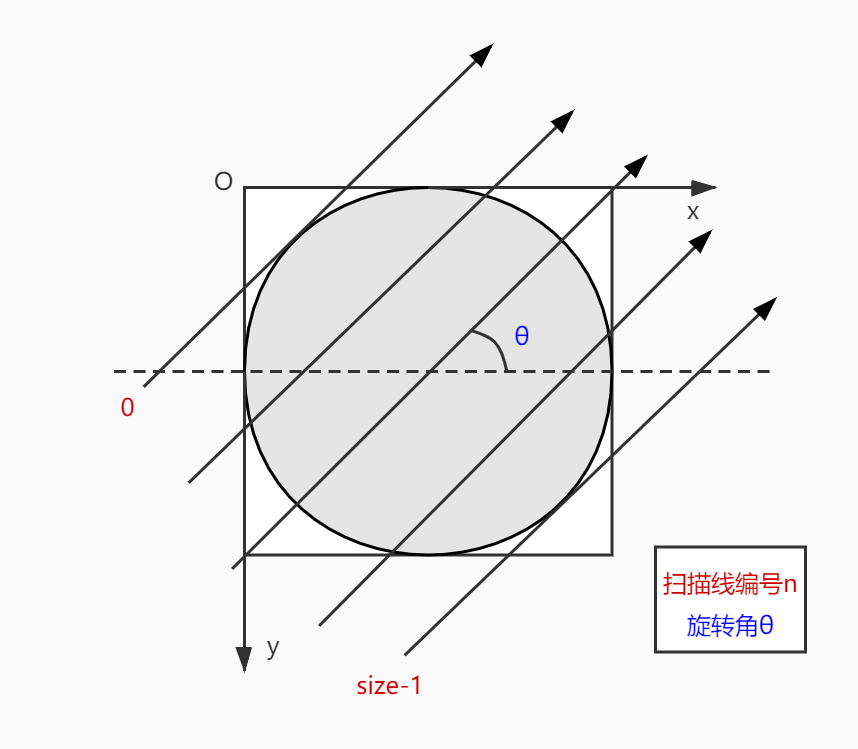
\includegraphics[width=0.7\textwidth]{../image/radon.jpg}
    \caption{Radon正变换实现}
    \label{fig Radon}
\end{figure}
其中最大的正方形表示待扫描的图像。我们默认扫描的区域范围用灰色部分显示。默认的扫描线方向如图中虚线所示,编号从上到下为[0,size-1]。扫描线与默认方向之间的夹角为$\theta$。设起始扫描线的坐标为$(x,y)$,则
% TODO 数学推导
\begin{equation}
    1324
\end{equation}
最后将每条扫描线上的值相加,就可以得到其中一个$theta$角所对应的扫描值,将其显示出来即可得到正弦图。

\subsection{Radon逆变换的实现}

\subsection{图形化界面的实现}

图形化界面采用了PySide2(PyQt)框架实现。UI文件储存在ui文件夹下,由两个页面组成,一个主页面和一个滤波反投影算法的参数选择界面。

\begin{figure}[H]
    \centering
    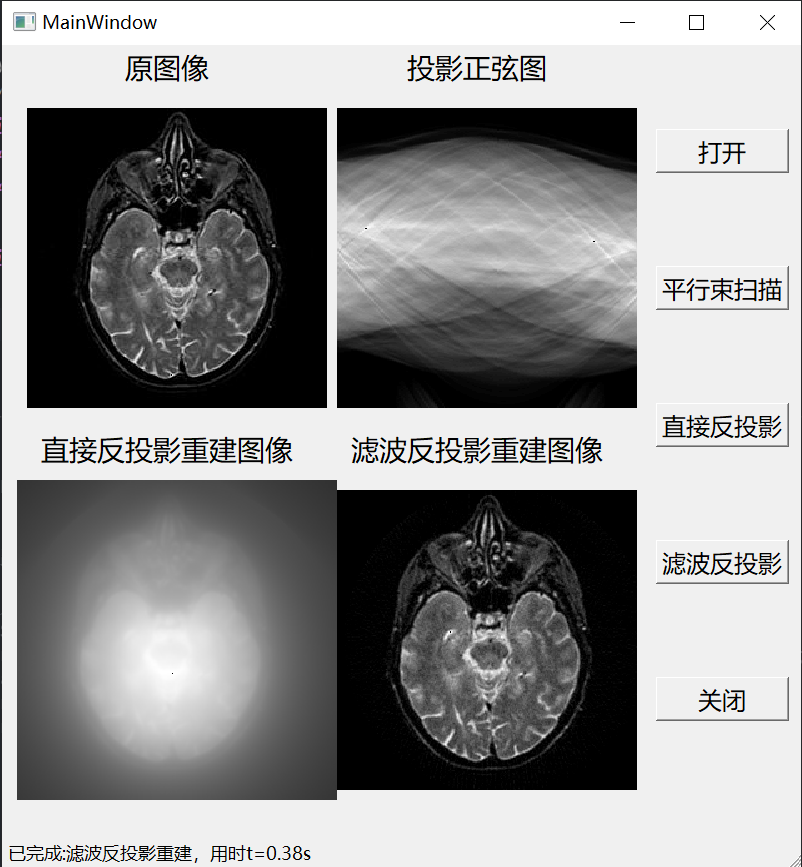
\includegraphics[width=0.7\textwidth]{../image/main_UI.png}
    \caption{主界面}
    \label{fig UI}
\end{figure}

本次实现的图形化界面具有以下几个特点:
\begin{itemize}
    \item 可以自行选择本地文件打开。
    \item 使用了多线程操作。图像处理等耗时的操作运行在另一个线程下,但是在计算过程中将页面上所有交互按钮禁用,防止用户进行误操作。
    \item 底部有状态栏,在运行过程中可以给予提示,运行结束后可以显示进行的操作和所消耗的时间。
    \item 在用户误操作时可以跳出错误提示。
\end{itemize}

\section{项目结果和评价}
\begin{figure}[H]
    \centering
    \includegraphics[width=\textwidth]{../image/visualize.png}
    \caption{CT图像重建结果}
    \label{fig reult}
\end{figure}
    


\section{感想与展望}

\end{document}
